\documentclass[UTF8]{ctexart}
%中文论文类型
%%%%preamble 定义导言开始%%%%%%%%%%%
\usepackage[greek,english]{babel}

\usepackage{amsmath}
\usepackage{float}
\usepackage{geometry}
\geometry{a6paper,centering,scale = 0.8}%%页面尺寸
\usepackage{graphicx}%%导入pdf/png/eps
\title{杂谈勾股定理}
\author{李世旺}
\date{\today}
\bibliographystyle{plain}%%声明参考文件格式
\newtheorem{thm}{定理}%%thm 变量
\newenvironment{myquote}{\begin{quote}\zihao{-6}\kaishu}{\end{quote}}
\newcommand\degree{^\circ}

%%%%preamble 定义导言结束%%%%%%%%%%%
\begin{document}
\maketitle
%制作标题
\begin{abstract}
这是一篇关于$\alpha$勾股定理\i\j($90\degree$)的小短文。
\end{abstract}
\tableofcontents
%制作目录
 \section{勾股定理在古代} 
 西方称勾股定理为毕达哥拉斯定理,
 将勾股定理的发现归功于公元前 6 世纪
 的毕达哥拉斯学派.该学派得到了一个法则,
 可以求出可排成直角三角形三边的\emph{三元数组}.
 
 毕达哥拉斯学派没有书面著作,该定理的严格表述和证明
 则见于欧几里德\footnote{欧几里德,约公元前 330--275 年。}《几何原本》的命题 47  :
 \begin{quote}
 \zihao{-3}\kaishu
 \emph{ “直角三角形斜边上
 的正方形等于两直角边上的 两个正方形之和。”}
 \end{quote}证明是用面积做的。
 \begin{equation}\label{eq:qqqqq}\angle ACB = \pi / 2 = 90^\circ\end{equation}
 
 
 
 \section{勾股定理的近代形式}
西方称勾股定理为毕达哥拉斯定理,
 将勾股定理的发现归功于公元前 6 世纪
 的毕达哥拉斯学派.该学派得到了一个法则,\begin{quote}可以求出可排成直角三角形三边的三元数组. \end{quote}
 毕达哥拉斯学派没有书面著作,该定理的严格表述和证明
 则见于欧几里德\footnote{欧几里德,约公元前 330--275 年。}《几何原本》的命题 47  :
 \begin{myquote}
 \emph{ “直角三角形斜边上
 的正方形等于两直角边上的 两个正方形之和。”}
 \end{myquote}证明是用面积做的。
 
 
 
 
 \section{方程式} 
 \begin{table}[H]
 \begin{tabular}{|r|r|r|}
\hline
直角边$a$&直角边$b$&直角边$c$\\
\hline
3&4&5\\
5&12&13\\
\hline
\end{tabular}%本注释会注释空格
\quad($a^2+b^2=c^2$)
\end{table}
 \begin{thm}[勾股定理]
直角三角形斜边的平方和等于两腰的平方和。\ref{eq:qqqqq}
\end{thm}
 \begin{thm}[判别式]
方程~$xy+zln~y+e^{xy} = 1. $ 
$$x_{\frac{-b \pm \sqrt{b^2 - 4ac}}{2a}\sqrt[3]{a}} = \frac{-b \pm \sqrt{b^2 - 4ac}}{2a}\sqrt[3]{a}$$
\end{thm}



\section{分式形式}
\begin{equation}
\Delta = b^2 - 4ac
\end{equation}
\begin{equation}x_{1,2} = \frac{-b \pm \sqrt{b^2 - 4ac}}{2a}\sqrt[3]{a}\end{equation}
\bibliographystyle{math}%%打印参考文件列表
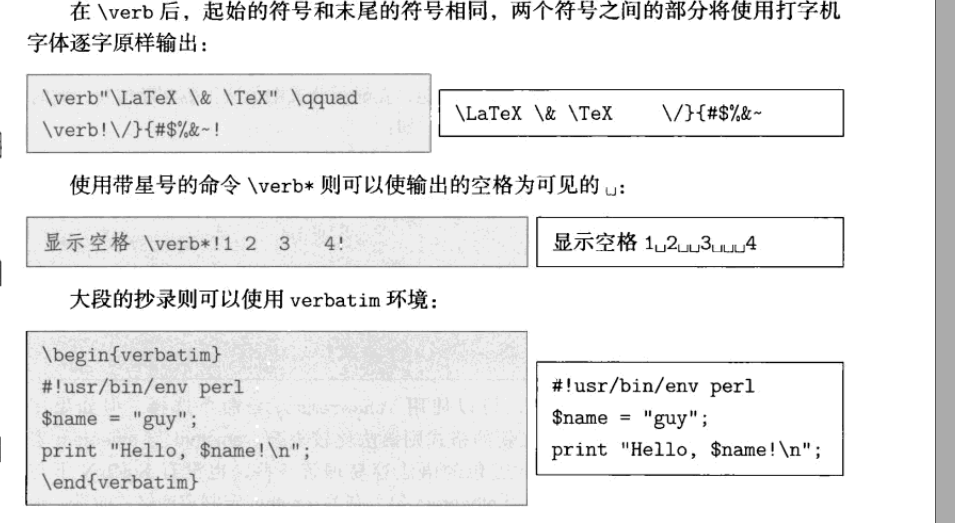
\includegraphics[scale = 0.3]{001.png}%%引用001.pdf首页
\end{document}